\documentclass{beamer}

\usepackage{amssymb}
\usepackage{amsmath}
\usepackage{amsfonts}
\usepackage{tikz}
\usepackage{xcolor}
\usepackage{graphicx}

\newcommand{\R}{\mathbb{R}}
\newcommand{\N}{\mathbb{N}}
\newcommand{\Q}{\mathbb{Q}}
\newcommand{\Z}{\mathbb{Z}}
\newcommand{\C}{\mathbb{C}}
\newcommand{\di}{\frac{dy}{dx}}
\newcommand{\dii}{\frac{d^2y}{dx^2}}
\newcommand{\din}{\frac{d^ny}{dx^n}}
\newcommand{\dt}{\frac{dx}{dt}}
\newcommand{\dtt}{\frac{d^2x}{dt^2}}
\newcommand{\dtn}{\frac{d^nx}{dt^n}}
\renewcommand{\vec}[1]{\underline{\textbf{#1}}}
\newcommand{\pd}[2]{\frac{\partial#1}{\partial#2}}
\newcommand{\fd}[2]{\frac{d #1}{d #2}}
\renewcommand{\l}{\lambda}
\newcommand{\g}{\gamma}
\renewcommand{\o}{\omega}
\newcommand{\el}{e^{\l x}}

%gets rid of navigation symbols
\setbeamertemplate{navigation symbols}{}

% LaTeX Tikz Flow Chart Commands 
\tikzstyle{startstop} = [rectangle, rounded corners, minimum width=2cm, minimum height=1cm,text centered, draw=black, fill=red!30]
\tikzstyle{io} = [trapezium, trapezium left angle=70, trapezium right angle=110, maximum width=2cm, minimum height=1cm, text centered, text width=3cm, draw=black, fill=blue!30]
\tikzstyle{process} = [rectangle, minimum width=3cm, minimum height=1cm, text centered, text width=6cm, draw=black, fill=orange!30]
\tikzstyle{decision} = [diamond, minimum width=2cm, minimum height=1cm, text centered, text width=6cm, draw=black, fill=green!30]
\tikzstyle{arrow} = [thick,->,>=stealth]

\usetikzlibrary{shapes.geometric, arrows}

\usepackage{tikz-3dplot}
\usetikzlibrary{shapes,calc,positioning,intersections}
\tdplotsetmaincoords{80}{120}

\title{On the revival of Navitus Bay}
\subtitle{An exploration into the mathematics of optimisation}
\author{Katie Murray, Ed Keall and James Arthur}
\date{Thursday 28th January 2020}


\usecolortheme{crane}
\setbeamertemplate{footline}{%
    \begin{beamercolorbox}[wd=\paperwidth,ht=2.25ex,dp=1ex,right, rightskip=1mm, leftskip=1mm]{titlelike}
        \inserttitle\hfill\insertauthor\hfill\insertframenumber%
    \end{beamercolorbox}
}

\setbeamertemplate{section in toc}[sections numbered]
\setbeamertemplate{subsection in toc}[subsections numbered]

\usepackage[backend=bibtex,style=authoryear]{biblatex}
\bibliography{./references.bib}

\begin{document}
\AtBeginSection[]
{
    \begin{frame}
        \frametitle{Table of Contents}
        \tableofcontents[currentsection]
    \end{frame}
}


\AtBeginSubsection[]
{
    \begin{frame}
        \frametitle{Table of Contents}
        \tableofcontents[currentsection,currentsubsection]
    \end{frame}
}

  \frame{\titlepage}

  \begin{frame}{Overview}
    \tableofcontents
  \end{frame}

  \section{Introduction}
  \begin{frame}
    \frametitle{Introduction}
    \begin{figure}[htp]
    \centering
    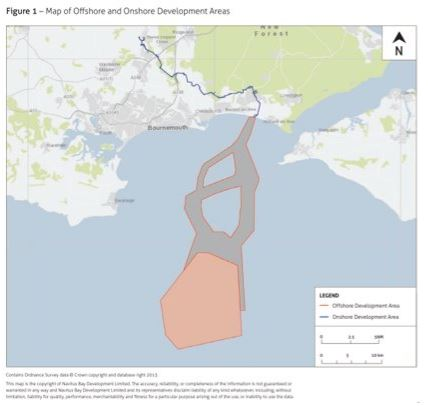
\includegraphics[width=.3\textwidth]{./figures/fig1.JPG}\hfill
    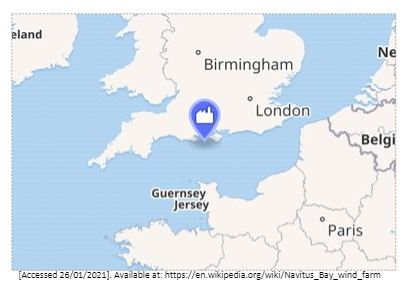
\includegraphics[width=.3\textwidth]{./figures/fig2.JPG}\hfill
    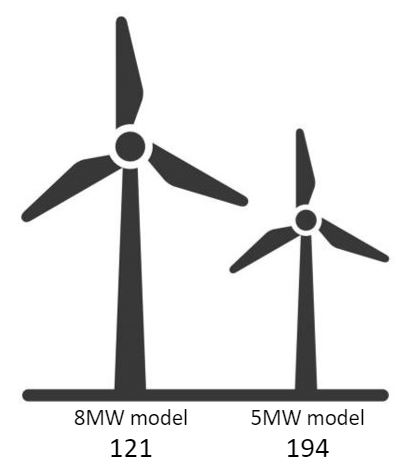
\includegraphics[width=.3\textwidth]{./figures/fig3.JPG}
    \label{fig:figure3}

    \end{figure}

    \begin{enumerate}
      \item Proposed power output capacity between $900$MW and $1200$MW.\pause
      \item Approximately $10$km south of Dorset.\pause
      \item Planning permission was refused in September 2015. \pause
      \item This gives us a proposed area of $196km^2$ and budget of 1.5 billion pounds.\autocite{navitus}
    \end{enumerate}
  \end{frame}

  \begin{frame}
    \frametitle{Our Optimisation Problem}
    Our problem is two fold,\pause
    \begin{enumerate}
      \item How many turbines should be in the Bay?\pause
      \item Where should they be placed?\pause
    \end{enumerate}
    Now we could refine these questions to be as fine as a hair, but our constraints which we will show, make clear what we are optimising against.
  \end{frame}

  \section{How many turbines?}
  \begin{frame}
    \frametitle{Constraints on number of turbines}
    \begin{table}[]
    \centering
    \resizebox{\textwidth}{!}{%
    \begin{tabular}{l|ll}
    \multicolumn{1}{c|}{}               & 8MW Turbine & 5MW Turbine  \\ \hline
    \multicolumn{1}{c|}{Rotor Diameter} & 167m        & 136m         \\
    Spacing                             & $1.074km^2$ & $0.7112km^2$ \\
    Cost                                & £4 million  & £2.5 million
    \end{tabular}%
    }
    \end{table}
  \end{frame}

\begin{frame}
  \frametitle{Single Objective LP}
  Let $x_1$ be number of $8$MW model turbines and $x_2$ be the number of $5$MW model turbines. \pause Now,
  $$ \max_{x} 8x_1 + 5x_2 $$
  $$ subject\,\, to \qquad\begin{matrix}
    0.34175\pi x_1 + 0.2265\pi x_2 \le 196\\
    4x_1 + 2.5x_2 \le 1500\\
    x_1 \ge 0\\
    x_2 \ge 0
  \end{matrix} $$\pause
  After implementing into MATLAB and using \texttt{intlinprog} we got the following solution. The optimal solution is 183 turbines with 181 being of the 8MW model and 2 of the 5MW model.
\end{frame}

\begin{frame}
  \frametitle{Feasible Region}
  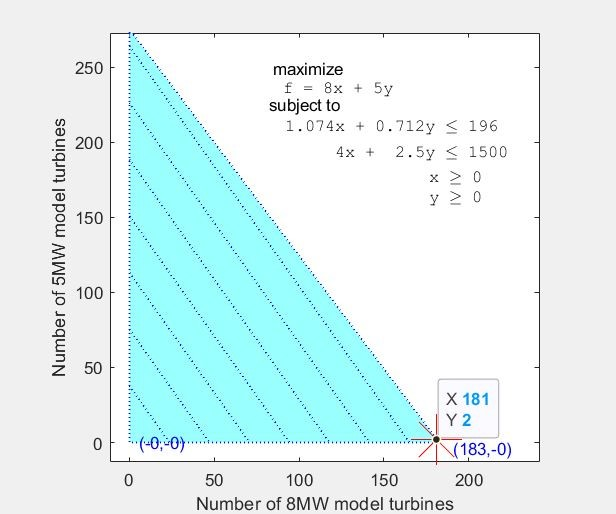
\includegraphics[width=0.9\linewidth]{./figures/fig4.jpg}
\end{frame}

\begin{frame}
  \frametitle{Multiobjective LP}
  
  Since, the cost constraint did not affect the feasible region (clear from the previous graph), we should instead aim to minimise the cost, and make cost another objective function, rather than a constraint. \pause
 
  Let $x_1$ be number of $8$MW model turbines and $x_2$ be the number of $5$MW model turbines. \pause Now,
  $$ \max_{x} 8x_1 + 5x_2 $$
  $$ \min_{x} 4x_1 + 2.5x_2 $$
  $$ subject\,\, to \qquad\begin{matrix}
    0.34175\pi x_1 + 0.2265\pi x_2 \le 196\\
    x_1 \ge 0\\
    x_2 \ge 0
  \end{matrix} $$\pause
  After implementing into MATLAB and using \texttt{fgoalattain} we got a set of solutions with a front.
\end{frame}


\begin{frame}
  \frametitle{Multiobjective Front}
  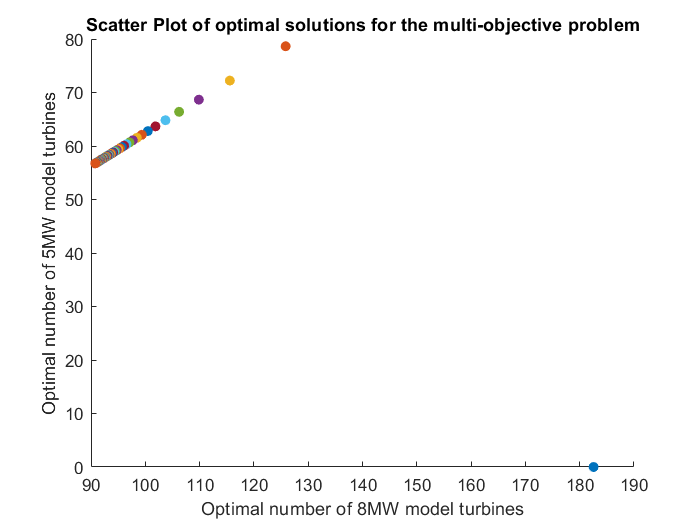
\includegraphics[width=0.9\textwidth]{./figures/fig5.png}
\end{frame}

\section{Where should they be placed?}
\subsection{Data}

\begin{frame}
  \frametitle{Data}
  \begin{figure}
    \begin{tikzpicture}[remember picture,overlay]
      \node[xshift=-8cm,yshift=-8cm] at (current page.north east) {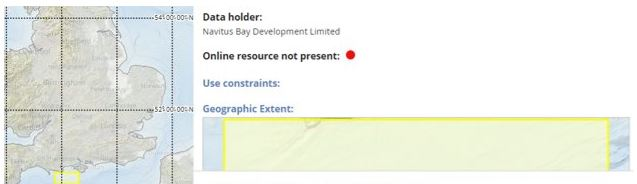
\includegraphics[width=0.8\textwidth]{./figures/fig7.jpg}};
    \end{tikzpicture}
    \begin{tikzpicture}[remember picture,overlay]
      \node[xshift=-3.2cm,yshift=-6.8cm] at (current page.north east) {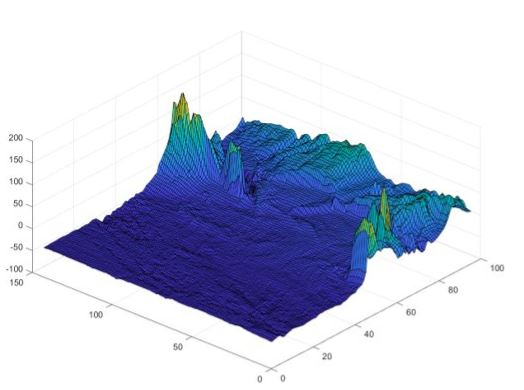
\includegraphics[width=0.6\textwidth]{./figures/fig6.jpg}};
    \end{tikzpicture}
  \end{figure}
  \vspace{-3cm}
  In order to know where to place turbines, we need data.\pause
  \begin{itemize}
    \item Unfortunately all the data collected from the Navitus Bay project wasn't available to us.\pause
    \item Bathemetry data was sourced from GEBCO \autocite{data}
  \end{itemize}
\end{frame}

\begin{frame}
  \frametitle{From Depth to Cost}
  \begin{figure}
    \begin{tikzpicture}[remember picture,overlay]
      \node[xshift=-10cm,yshift=-7cm] at (current page.north east) {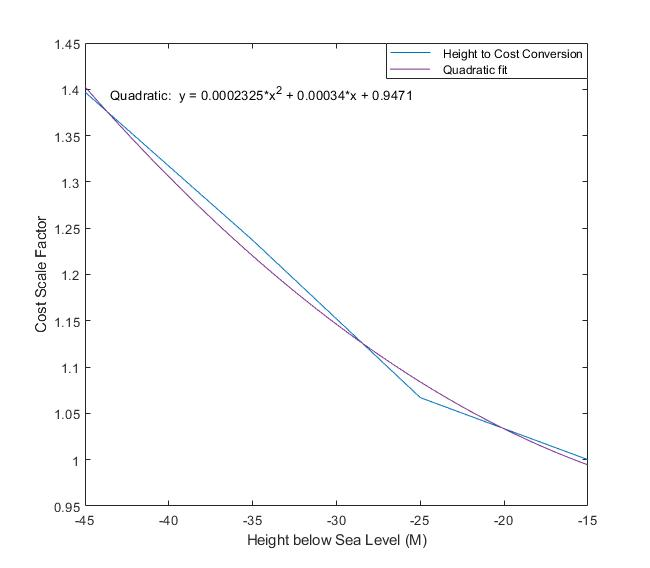
\includegraphics[width=0.5\textwidth]{./figures/fig9.jpg}};
    \end{tikzpicture}
    \begin{tikzpicture}[remember picture,overlay]
      \node[xshift=-3cm,yshift=-7cm] at (current page.north east) {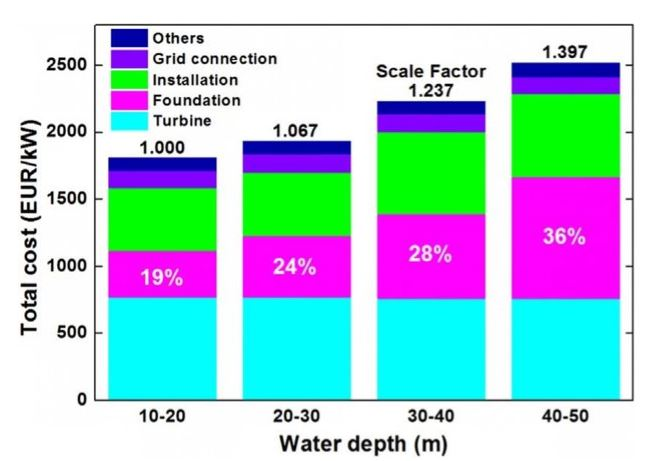
\includegraphics[width=0.5\textwidth]{./figures/fig10.jpg}};
    \end{tikzpicture}
  \end{figure}
  \vspace{-4cm}
  \begin{itemize}
    \item Using data from a paper on offshore wind turbine costs, we created a quadratic model from depth to cost.\autocite{data_paper}\pause
    \item Using this model the bathymetry dataset was changed to show cost of location.
  \end{itemize}
\end{frame}

\begin{frame}
  \frametitle{Conversion of Map to Metric}
  \begin{figure}
    \begin{tikzpicture}[remember picture,overlay]
      \node[xshift=-6cm,yshift=-7cm] at (current page.north east) {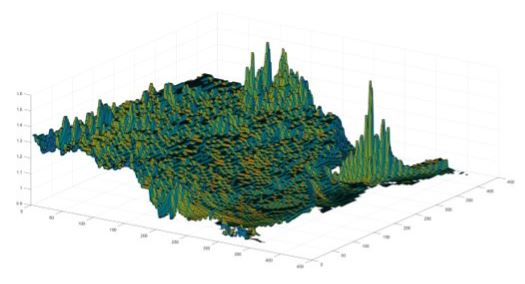
\includegraphics[width=0.61\textwidth]{./figures/fig11.jpg}};
    \end{tikzpicture}
  \end{figure}
  \vspace{-3cm}
  \begin{itemize}
    \item Bathymetry Dataset grid from GEBCO is irregular using longitude and latitude instead of meters.\pause
    \item Each cell was approximately 291m $\times$ 458m.\pause
    \item We created a new matrix from each cell, of each 29m $\times$ 46m to be combined into a matrix of 10m $\times$ 10m cells.\pause
    \item To reduce processing, this matrix was averaged to 100m $\times$ 100m cells
  \end{itemize}
\end{frame}

\subsection{Algorithmic Placement}

\begin{frame}
  \frametitle{Random Placement}
    \begin{figure}
      \begin{tikzpicture}[remember picture,overlay]
        \node[xshift=-3cm,yshift=-7cm] at (current page.north east) {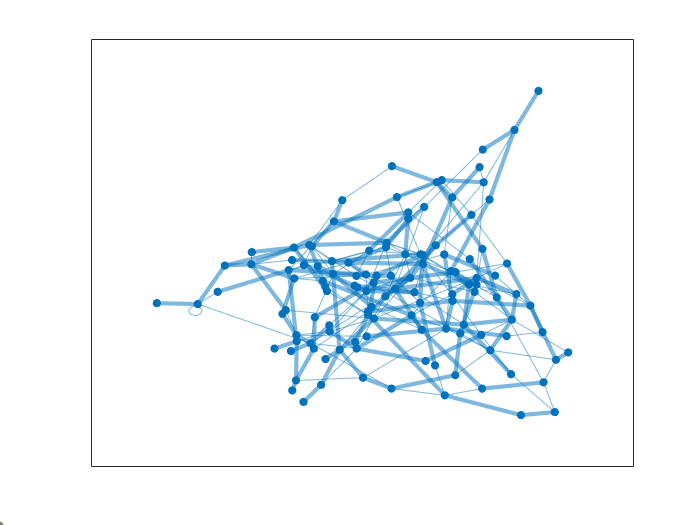
\includegraphics[width=0.5\textwidth]{./figures/fig12.png}};
      \end{tikzpicture}

      \begin{tikzpicture}[remember picture,overlay]
        \node[xshift=-9cm,yshift=-7.5cm] at (current page.north east) {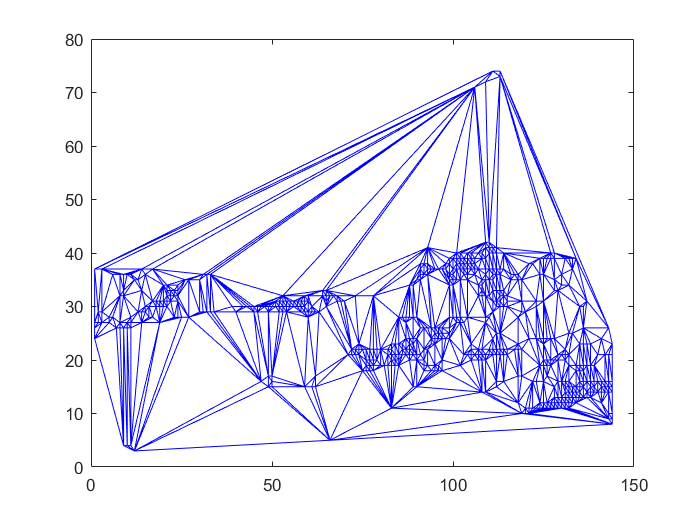
\includegraphics[width=0.45\textwidth]{./figures/fig13.png}};
      \end{tikzpicture}
    \end{figure}
  \begin{itemize}
    \vspace{-4cm}
    \item The first thing that we tried was a randomised approach, choose points at random and create a minimum spanning tree off that.\pause
    \item This then lead to some ideas and rabbit holes of potentially using Perlin noise, Delaunay triangulation or sphere packing algorithms to aid the placement. However we decided using actual data was the best cause of action.\pause
    \item We then started programming\\ an algorithm.
  \end{itemize}
\end{frame}

\begin{frame}{The Algorithm}
  \begin{figure}
      \centering
      \begin{tikzpicture}[node distance=1.5cm]
        \node (start) [startstop] {Start};
        \node (in1) [io, below of=start] {$n$ points where cost is lowest};
        \node (pro1) [process, below of=in1] {Calculate center point and calculate centralisation factor.};
        \node (pro2) [process, below of=pro1] {Make Adjacency Matrix and find all of the right distanced points};
        \node (out1) [io, below of=pro2] {Output weighted average};
        \node (stop) [startstop, right of=out1, xshift=3cm] {Stop};
        \draw [arrow] (start) -- (in1);
        \draw[arrow] (in1) -- (pro1);
        \draw[arrow] (pro1) -- (pro2);
        \draw[arrow] (pro2) -- (out1);
        \draw[arrow] (out1) -- (stop);
      \end{tikzpicture}
      \caption{The Algorithm for finding optimal placement}
      \label{fig:algo}
  \end{figure}
\end{frame}

\begin{frame}
  \begin{figure}
    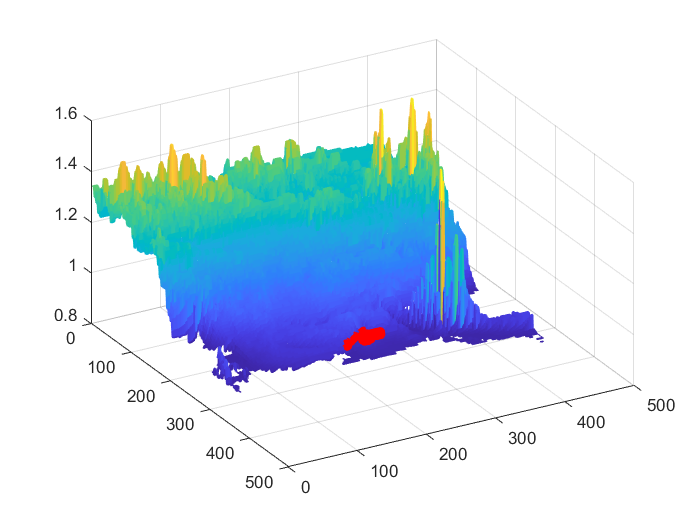
\includegraphics[width=0.9\textwidth]{./figures/fig14.png}
    \caption{A not quite perfect plot of the surface}
  \end{figure}
\end{frame}

\begin{frame}{The  New Updated Algorithm}
  \begin{figure}
      \centering
      \begin{tikzpicture}[node distance=1.5cm]
        \node (start) [startstop] {Start};
        \node (in1) [io, below of=start] {$n$ {\color{red}\textbf{randomly distributed}} points};
        \node (pro1) [process, below of=in1] {Calculate center point and calculate centralisation factor.};
        \node (pro2) [process, below of=pro1] {Make Adjacency Matrix and find all of the right distanced points};
        \node (out1) [io, below of=pro2] {Output weighted average};
        \node (stop) [startstop, right of=out1, xshift=3cm] {Stop};
        \draw [arrow] (start) -- (in1);
        \draw[arrow] (in1) -- (pro1);
        \draw[arrow] (pro1) -- (pro2);
        \draw[arrow] (pro2) -- (out1);
        \draw[arrow] (out1) -- (stop);
      \end{tikzpicture}
      \caption{The Algorithm for finding optimal placement}
      \label{fig:algo}
  \end{figure}
\end{frame}

\begin{frame}
  \begin{figure}
    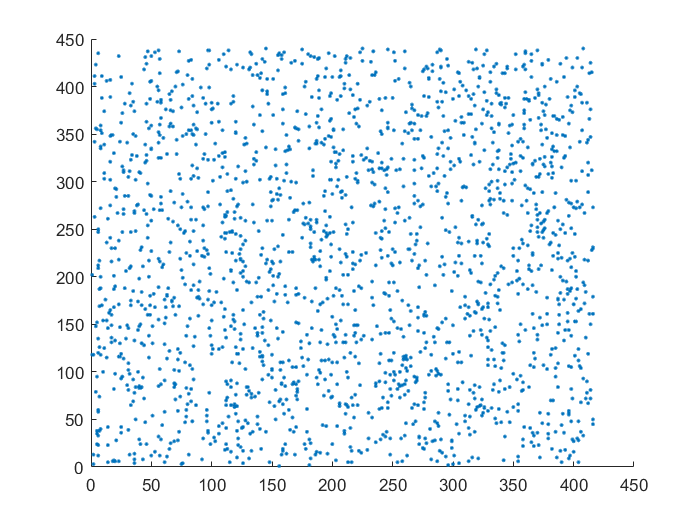
\includegraphics[width=0.9\textwidth]{./figures/fig17.png}
    \caption{2000 Points of uniform placement over the seabed.}
  \end{figure}
\end{frame}

\begin{frame}
  \begin{figure}
    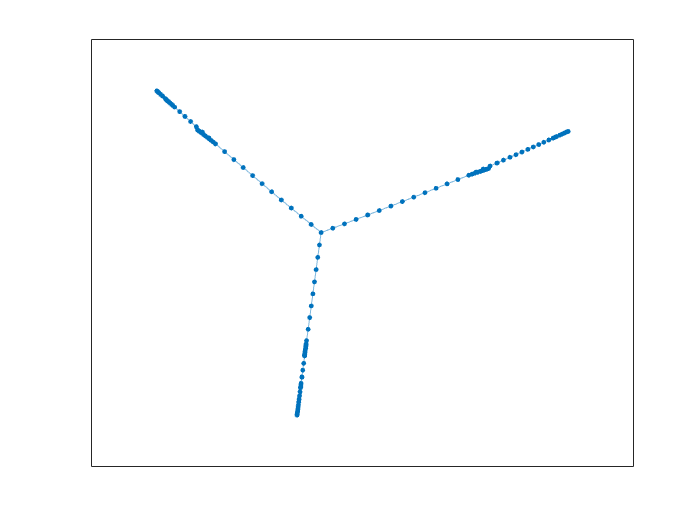
\includegraphics[width=0.9\textwidth]{./figures/fig19.png}
    \caption{The MST of all the optimal points.}
  \end{figure}
\end{frame}

\begin{frame}
  \begin{figure}
    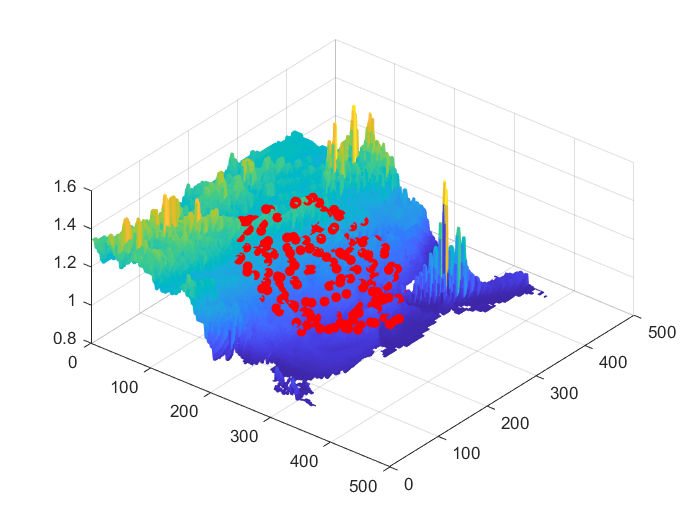
\includegraphics[width=0.9\textwidth]{./figures/fig15.png}
    \caption{The locations of the optimal points on the surface}
  \end{figure}
\end{frame}
\begin{frame}
  \begin{figure}
    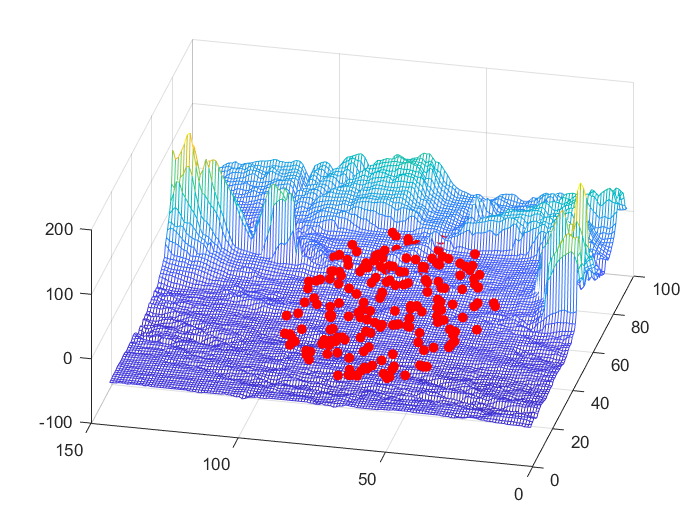
\includegraphics[width=0.9\textwidth]{./figures/fig18.png}
    \caption{The points of optimal placement for the 183 turbines}
  \end{figure}
\end{frame}

\section{Conclusion}

\begin{frame}
  \frametitle{Conclusion}
  \begin{itemize}
    \item After a few weeks we have found optimal number of different for the turbines, 181 big turbines and 2 small with respect to cost. \\\pause
    \item We also found the optimal spacing of them in the bay, with respect to relevant physical factors.\\\pause
    \item If given more time we could implement an `annoyance' factor, which have the mathematics of, but omitted as it wasn't included in the code. \\\pause
    \item Even though we may not see Navitus Bay come to fruition, it is still a lovely mathematical problem to explore optimisation with.\qed
  \end{itemize}
\end{frame}

\begin{frame}
  \frametitle{References}
  \printbibliography
\end{frame}
\end{document}
